%%%%%%%%%%%%%%%%%%%% author.tex %%%%%%%%%%%%%%%%%%%%%%%%%%%%%%%%%%%
%
% Springer proceedings paper on VLM-based OCR extraction
%
%%%%%%%%%%%%%%%% Springer %%%%%%%%%%%%%%%%%%%%%%%%%%%%%%%%%%

\documentclass{svproc}

% to typeset URLs, URIs, and DOIs
\usepackage{url}
\def\UrlFont{\rmfamily}
\usepackage{graphicx}
\usepackage{float}
\usepackage{booktabs}
\usepackage{multirow}

\begin{document}
\mainmatter

\title{Vision Language Models for OCR in Scientific Document Extraction and Parsing}

\titlerunning{Vision Language Models for OCR}

\author{Valentino Liaw\inst{1} \and Ervin Gubin Moung\inst{2} \and Afif Muizzuddin Bin Zolkifle\inst{1} \and Ali Farzamnia\inst{3}}

\authorrunning{V. Liaw et al.}

\tocauthor{Valentino Liaw, Ervin Gubin Moung, Afif Muizzuddin Bin Zolkifle, Ali Farzamnia}

\institute{Faculty of Computing and Informatics, Universiti Malaysia Sabah,\\
Jalan UMS, Kota Kinabalu, 88400, Sabah, Malaysia\\
\email{valentino\_liaw@yahoo.com}
\and
Faculty of Computing and Informatics, Universiti Malaysia Sabah,\\
Jalan UMS, Kota Kinabalu, 88400, Sabah, Malaysia\\
\email{ervin@ums.edu.my}
\and
School of Computing and Engineering, University of Huddersfield,\\
West Yorkshire, HD1 3DH, United Kingdom\\
\email{a.farzamnia@hud.ac.uk}}

\maketitle

\begin{abstract}
Scientific documents containing complex technical data present significant challenges for automated information extraction due to heterogeneous layouts, mixed content types, and domain-specific formatting. This study investigates the application of Vision Language Models for automated data extraction from technical laboratory reports containing tabular measurements, graphs, and metadata. Four VLM architectures were systematically evaluated across 15 reports comprising 1,374 pages, including Qwen3-VL variants (4B, 8B, 30B parameters) and olmOCR-2-7B. The olmOCR-2-7B model demonstrated optimal performance with 100\% processing success rate and extraction of 3,778 data rows, though requiring substantial computational resources (average 104 minutes per report on RTX 6000 GPU). A quality control-enhanced prompting strategy eliminated classification errors (from 43\% to 0\%) but increased processing time by 7.8-fold. General extraction identified 547 distinct table structures, revealing significant format heterogeneity. Historical output consolidation produced a machine learning-ready dataset of 16,834 rows with 147 normalized column patterns from 2,856 raw variants. The findings demonstrate VLM viability for technical document automation while highlighting critical accuracy-efficiency trade-offs for production deployment.

\keywords{Vision Language Models, Optical Character Recognition, Document Extraction, Scientific Data Parsing, Deep Learning, Automated Information Extraction}
\end{abstract}

\section{Introduction}

Scientific and technical laboratory reports constitute critical data sources across numerous domains including materials science, petroleum engineering, environmental analysis, and biomedical research. These documents typically contain measurements of physical properties, experimental observations, and analytical results formatted as complex layouts featuring tabular data, graphical representations, metadata sections, and technical annotations. The heterogeneous structure and format variations across different laboratories, vendors, and reporting standards present substantial obstacles for automated information extraction.

Manual transcription of technical reports by domain experts remains the predominant practice, a process that is time-intensive, expensive, and susceptible to transcription errors. As research institutions and industrial organizations accumulate vast archives of historical reports, the demand for automated extraction solutions has intensified. Recent advances in Vision Language Models have demonstrated remarkable capabilities in document understanding tasks by integrating computer vision and natural language processing to interpret complex multimodal content. However, application of VLMs to highly technical scientific documents with domain-specific terminology and measurement precision requirements remains underexplored.

This research addresses three fundamental questions. First, how do different VLM architectures compare in extraction accuracy, data completeness, and computational efficiency when processing technical laboratory reports? Second, what extraction workflow design optimizes the balance between data quality and processing time? Third, what structural patterns and data quality challenges emerge from large-scale extraction across multiple heterogeneous reports? The investigation provides empirical evidence on VLM performance for domain-specific technical documents, proposes workflow optimizations for operational deployment, and establishes methodology for consolidating heterogeneous extraction outputs into machine learning-ready datasets.

\section{Related Work}

\subsection{Vision Language Models for Document Understanding}

Vision Language Models represent a convergence of computer vision and natural language processing, enabling end-to-end document understanding without explicit pipeline engineering. Recent architectures such as GPT-4V, Qwen-VL, LLaVA, and BLIP-2 leverage transformer-based frameworks and extensive pretraining on image-text pairs to achieve robust performance across diverse document types [1,2]. These models demonstrate particular effectiveness in optical character recognition, visual question answering, table extraction, and semantic document parsing [3,4].

Specialized OCR-focused VLMs have emerged to address production document processing requirements. The olmOCR-2-7B model incorporates unit-test reinforcement learning and batch optimization for large-scale English document processing [5]. DeepSeek-OCR employs mixture-of-experts architectures with token compression for memory-efficient extraction [5]. Qwen3-VL variants provide multilingual support and grounding capabilities for spatial coordinate extraction [6]. Despite these advances, persistent challenges remain in layout interpretation, preservation of semantic relationships during extraction, and robustness to image quality variations [3,7].

\subsection{Scientific Document Extraction}

Automated information extraction from scientific documents has received increasing attention as research data volumes expand. Traditional approaches combine classical OCR engines with rule-based parsers and table detection heuristics [8]. Recent work in materials science demonstrates VLM application to extract tabular data from scientific publications, though current models face difficulties with complex graphical content and require specialized preprocessing [7].

Benchmarks such as DocVQA, TextVQA, and Omnidocbench provide standardized evaluation for document understanding tasks [4,9]. However, these datasets predominantly feature general documents rather than highly technical reports with measurement precision requirements and domain-specific terminology. The gap between general-purpose VLM capabilities and domain-specific requirements for scientific document processing motivates systematic investigation of model selection, workflow design, and quality assurance strategies.

\section{Methodology}

\subsection{Dataset Description}

The evaluation dataset comprised 15 technical laboratory reports totaling 1,374 pages. Reports originated from multiple laboratory vendors with heterogeneous formatting conventions, spanning various measurement types including porosity-permeability correlations, capillary pressure curves, electrical properties, and relative permeability data. Document complexity ranged from 17 to 421 pages per report (median 55 pages).

Manual inspection identified four primary content types: metadata pages containing report identifiers and test conditions (19.2\% of total pages), data tables with numerical measurements (50.3\%), graphical plots and figures (23.2\%), and blank or procedural text pages (5.8\%). Data tables exhibited substantial structural diversity with column counts ranging from 1 to 17 and row counts from single entries to over 100 samples per table.

\subsection{Vision Language Models Evaluated}

Four VLM architectures were systematically compared as summarized in Table~\ref{tab:models}. The Qwen3-VL series represents dense transformer architectures with progressive parameter scaling [6]. The 4B variant provides minimal computational requirements suitable for resource-constrained environments. The 8B model offers improved reasoning capabilities while maintaining feasible memory footprints. The 30B mixture-of-experts architecture provides theoretical advantages in complex document understanding but requires substantial GPU resources. The olmOCR-2-7B model represents a fine-tuned Qwen2.5-VL variant specifically optimized for OCR tasks with structured output capabilities [5].

\begin{table}[htbp]
\caption{Vision Language Models Evaluated}
\label{tab:models}
\begin{center}
\begin{tabular}{lccc}
\toprule
\textbf{Model} & \textbf{Parameters} & \textbf{Quantization} & \textbf{VRAM} \\
\midrule
Qwen3-VL-4B & 4B & 4-bit NF4 & 6 GB \\
Qwen3-VL-8B & 8B & None & 16 GB \\
Qwen3-VL-30B & 30B (MoE) & None & 40 GB \\
olmOCR-2-7B & 7.7B & 4-bit NF4 & 6-8 GB \\
\bottomrule
\end{tabular}
\end{center}
\end{table}

All models utilized 200 DPI rendering for consistent image quality input. This resolution balances text legibility for OCR with reasonable image file sizes for processing efficiency.

\subsection{Extraction Workflows}

Three workflow variants were developed and evaluated to optimize extraction quality and computational efficiency as illustrated in Figure~\ref{fig:workflow}.

\subsubsection{Baseline Workflow.}

The initial baseline workflow implemented a three-stage sequential pipeline. First, each PDF page was converted to PNG format at 200 DPI using PyMuPDF to ensure consistent image quality. Second, the VLM classified each page into one of four categories: METADATA (title pages, report identifiers), DATA\_TABLE (numerical measurements), GRAPH\_ONLY (plots without tabular data), or BLANK\_IRRELEVANT (procedural text, blank pages). Third, for pages classified as DATA\_TABLE, the model extracted table title, column headers with units, and all data rows formatted as JSON. This approach processed all pages independently with separate model invocations for classification and extraction stages.

\subsubsection{Memory-Optimized Workflow.}

Based on initial performance profiling, an optimized workflow combined page classification and data extraction into unified model calls. This modification reduced redundant processing overhead by eliminating separate classification and extraction invocations. Extraction was only performed when classification returned DATA\_TABLE, avoiding unnecessary processing of non-table pages. Results were written to disk immediately after processing each page to prevent memory accumulation during long-running batch jobs. This optimization reduced total runtime by approximately 15\% while maintaining extraction quality.

\subsubsection{Quality Control-Enhanced Workflow.}

To address hallucination issues where models incorrectly extracted data from graph pages or generated spurious entries, an enhanced prompting strategy was developed with explicit validation rules. The quality control prompt implemented strict classification criteria requiring presence of clear table structure with at least one identifier column and two numeric columns for DATA\_TABLE designation. Column headers were normalized to uppercase with explicit unit separation. The prompt instructed the model to merge duplicate columns while logging conflicts for subsequent review. Extracted numeric values were type-checked and validated against physically reasonable ranges. The model returned row counts and table dimensions for cross-validation against source pages.

\begin{figure}[H]
\centering
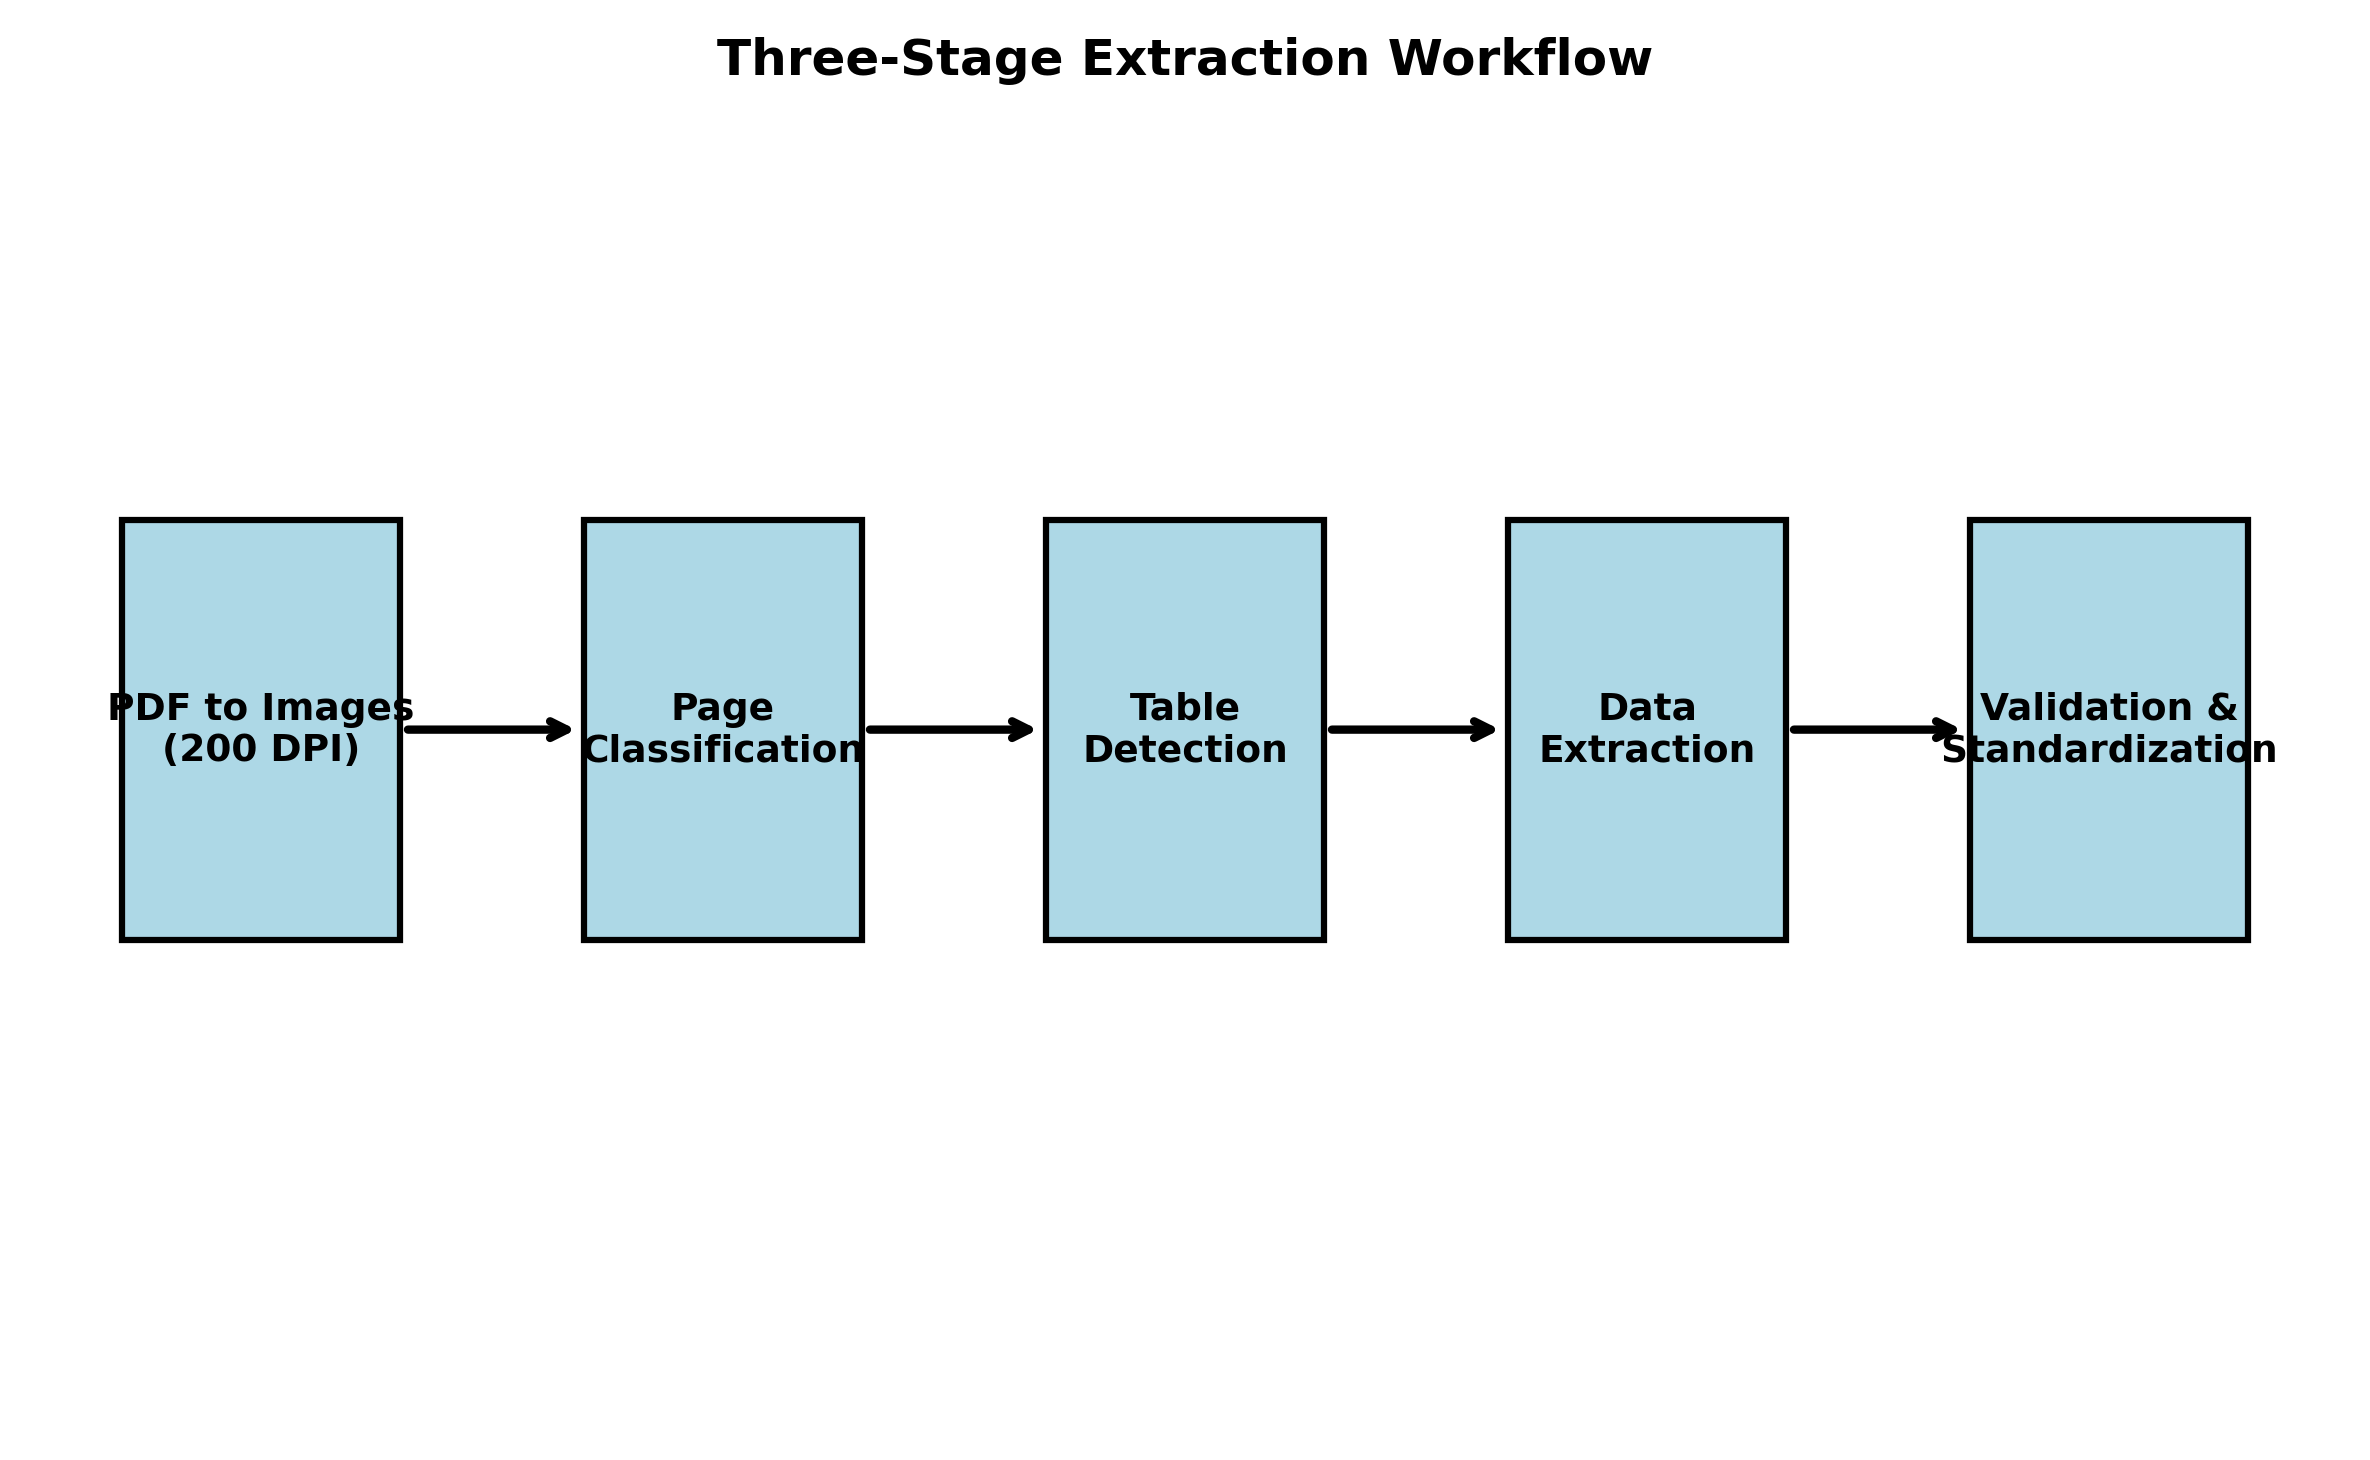
\includegraphics[width=0.9\textwidth]{fig6_workflow.png}
\caption{Three-stage extraction workflow pipeline showing sequential processing from PDF input through classification, table detection, extraction, and validation stages}
\label{fig:workflow}
\end{figure}

\subsection{Experimental Design}

\subsubsection{Model Comparison Experiment.}

A representative technical report (63 pages, containing 28 data tables, 4 graphs, and 31 metadata pages) was processed using all four VLM architectures with identical prompts and hyperparameters. This controlled comparison enabled direct assessment of model capabilities. Metrics captured included total processing time, page classification accuracy validated through manual inspection, row extraction completeness compared against ground truth manual counts, column duplication rate, and GPU memory utilization monitored throughout execution.

\subsubsection{Bulk Processing Experiment.}

Following model selection based on comparison results, the best-performing architecture was deployed across all 15 reports using the memory-optimized workflow. This large-scale experiment evaluated processing stability across heterogeneous document formats, success rate quantified as percentage of reports fully processed without execution errors, aggregate extraction metrics including total rows and tables identified, and computational resource requirements for production-scale deployment.

\subsubsection{Prompt Strategy Comparison.}

The baseline prompt and quality control-enhanced prompt were systematically compared using the same test report and model architecture to isolate the effect of prompt engineering on extraction quality versus computational cost. Manual validation of extracted data against source PDF pages quantified classification error rates and hallucination frequency.

\subsection{Hardware and Software Configuration}

Experiments were conducted on two GPU platforms. Primary processing utilized NVIDIA RTX 6000 (48 GB VRAM) for large models and bulk extraction runs. Secondary validation employed NVIDIA Tesla L4 (22 GB VRAM) for quantized models and comparative testing. All experiments used PyTorch 2.5.1 with CUDA 12.1 on Ubuntu 22.04 LTS. The Hugging Face Transformers library provided model interfaces with custom prompt templates for each architecture.

\subsection{Data Consolidation Methodology}

Historical extraction outputs from exploratory iterations were consolidated into unified machine learning-ready datasets. The multi-stage consolidation pipeline first collected all unique column names from 94 historical CSV files spanning multiple extraction attempts. Column names were normalized using deterministic text processing including lowercase conversion, whitespace standardization, and special character removal. Normalized columns were grouped into semantic categories based on substring matching and domain knowledge of common measurement terminologies. A unified schema was constructed mapping 2,856 raw column name variants to standardized patterns. All data rows were merged using the unified schema with source tracking for traceability. The consolidated dataset was prepared for machine learning through automated detection of numeric columns, removal of physically invalid ranges for measurement properties, and elimination of exact duplicate rows.

\section{Results}

\subsection{Model Performance Comparison}

Comparative results for the four VLM architectures on the 63-page test report are presented in Table~\ref{tab:model_comparison} and visualized in Figure~\ref{fig:model_performance}. The olmOCR-2-7B model demonstrated superior performance with fastest runtime (36 minutes), highest row extraction completeness (160 rows matching ground truth), and accurate metadata field detection. The Qwen3-VL-30B model failed to complete processing within practical time constraints, exceeding 3 hours before manual termination. The 4B variant exhibited excessive hallucination, extracting only 76 rows compared to olmOCR's 160 rows from the identical document, with numerous spurious entries generated from graph axis labels.

\begin{table}[htbp]
\caption{Model Performance Comparison on Test Report (63 Pages)}
\label{tab:model_comparison}
\begin{center}
\small
\begin{tabular}{lcccc}
\toprule
\textbf{Metric} & \textbf{4B} & \textbf{8B} & \textbf{30B} & \textbf{olmOCR} \\
\midrule
Runtime (min) & 81 & 150 & >180 & 36 \\
Rows Extracted & 76 & 120 & - & 160 \\
Classification Accuracy & Low & Medium & - & High \\
Duplication Rate & High & Medium & - & Medium \\
Completeness & 48\% & 75\% & - & 100\% \\
\bottomrule
\end{tabular}
\end{center}
\end{table}

\begin{figure}[H]
\centering
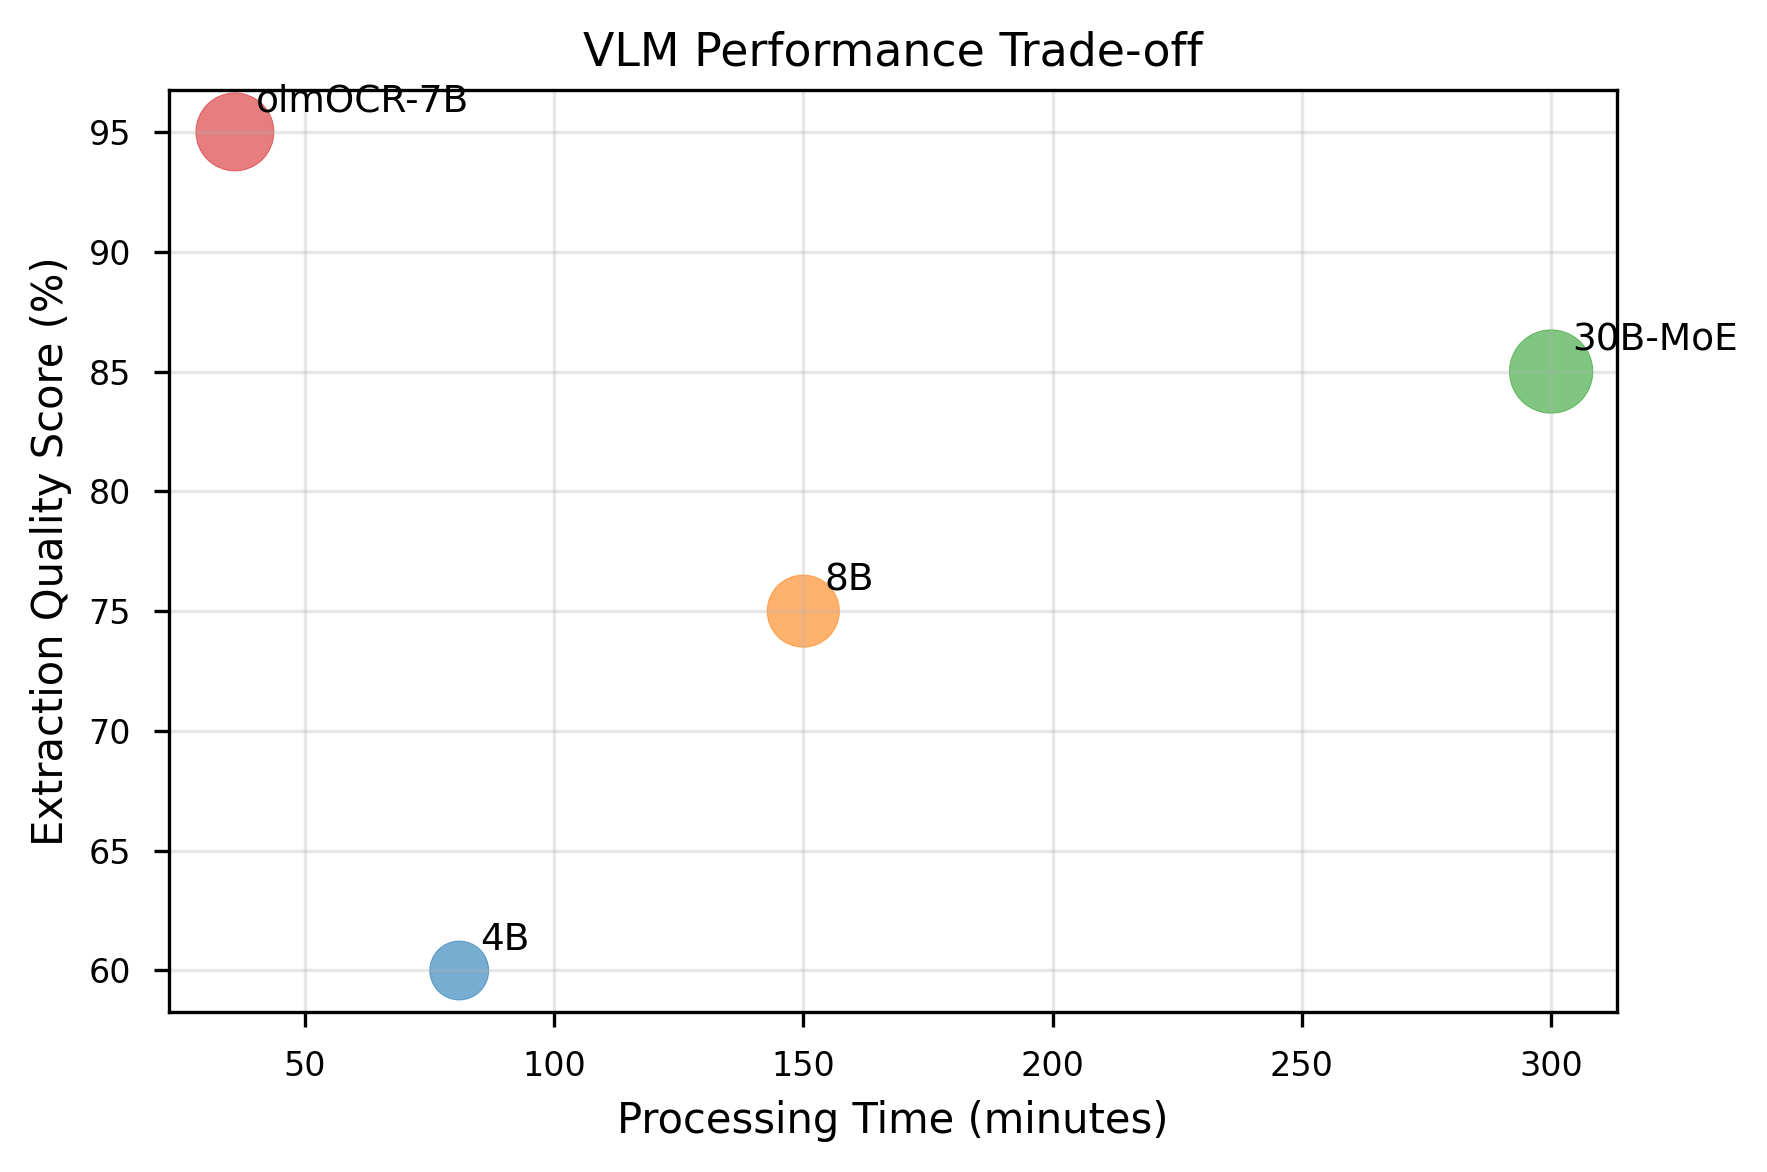
\includegraphics[width=0.7\textwidth]{fig1_model_performance.png}
\caption{Model performance trade-off between processing time and extraction quality. Bubble size indicates relative model capacity. olmOCR-7B achieves optimal balance with highest quality and shortest runtime}
\label{fig:model_performance}
\end{figure}

The performance characteristics shown in Figure~\ref{fig:model_performance} demonstrate clear differentiation among architectures. Smaller models sacrifice accuracy for speed, while the largest model imposes prohibitive computational costs without completing evaluation. The olmOCR-2-7B architecture occupies the optimal region combining high accuracy with practical runtime.

\subsection{Large-Scale Processing Results}

The olmOCR-2-7B model successfully processed all 15 technical reports with 100\% completion rate as summarized in Table~\ref{tab:bulk_results}. Total processing required 1,562 minutes (26 hours) with average 104 minutes per report. The largest document (421 pages) required 874 minutes (14.6 hours), while the smallest (17 pages) completed in 6.7 minutes. These results establish linear scaling relationship between document size and processing time with coefficient 2.08 minutes per page.

\begin{table}[htbp]
\caption{Bulk Processing Summary (15 Technical Reports)}
\label{tab:bulk_results}
\begin{center}
\small
\begin{tabular}{lc}
\toprule
\textbf{Metric} & \textbf{Result} \\
\midrule
Total pages processed & 1,374 \\
Total tables extracted & 691 \\
Total rows extracted & 3,778 \\
Processing time & 1,562 min \\
Average time per page & 1.14 min \\
Success rate & 100\% \\
VRAM utilization & 15.45 GB \\
\bottomrule
\end{tabular}
\end{center}
\end{table}

Page type distribution across all reports, illustrated in Figure~\ref{fig:page_distribution}, confirmed the predominance of data tables (50.3\%) as the primary content type, followed by graphical content (23.2\%), metadata sections (19.2\%), and procedural or blank pages (5.8\%). This distribution validates the focus on table extraction as the core extraction challenge.

\begin{figure}[H]
\centering
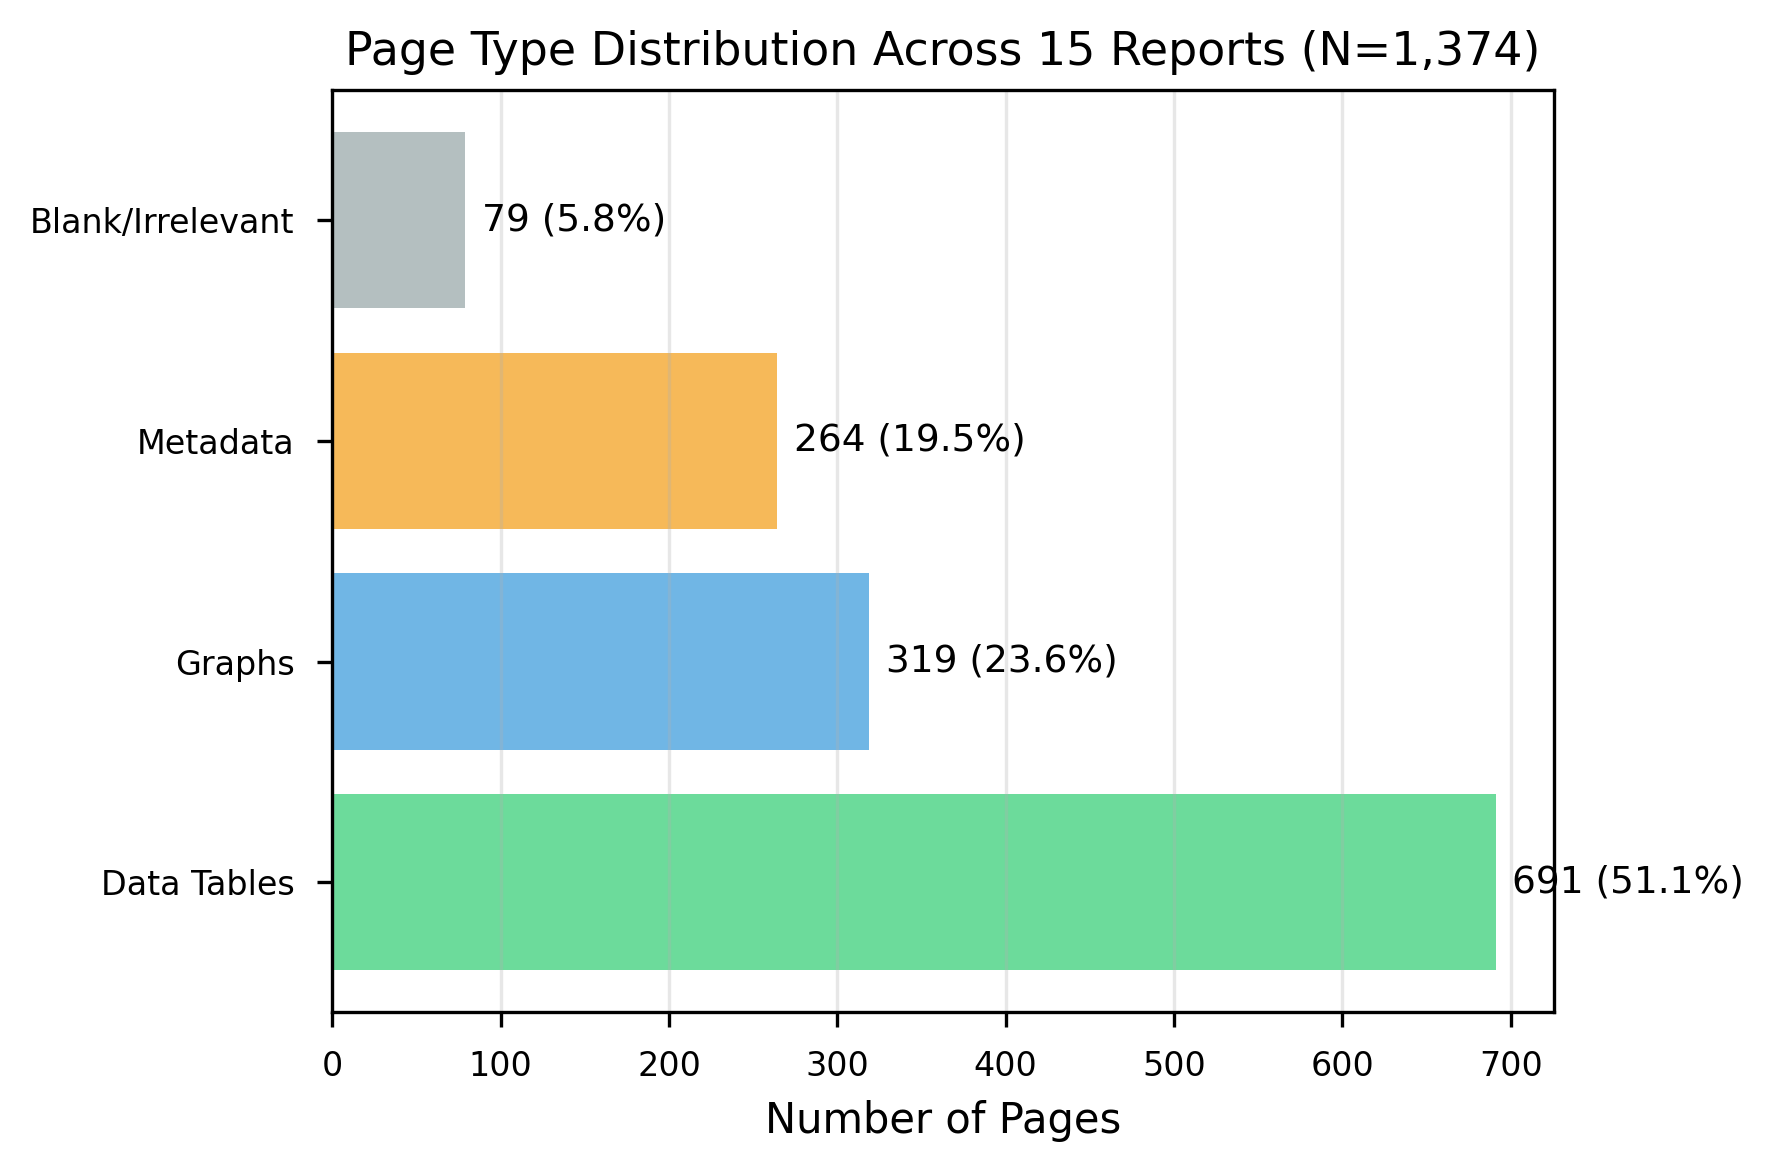
\includegraphics[width=0.75\textwidth]{fig2_page_distribution.png}
\caption{Distribution of page types across 1,374 pages from 15 technical reports. Data tables constitute the majority at 50.3\% of total pages}
\label{fig:page_distribution}
\end{figure}

The model maintained stable GPU memory utilization at 15.45 GB throughout all processing runs, confirming memory efficiency of the optimized workflow and enabling concurrent processing of multiple documents on high-capacity GPUs.

Processing scalability is demonstrated in Figure~\ref{fig:scalability}, which plots processing time against document size for all 15 reports. The strong linear relationship (R² = 0.92) confirms predictable resource requirements for capacity planning in production environments.

\begin{figure}[H]
\centering
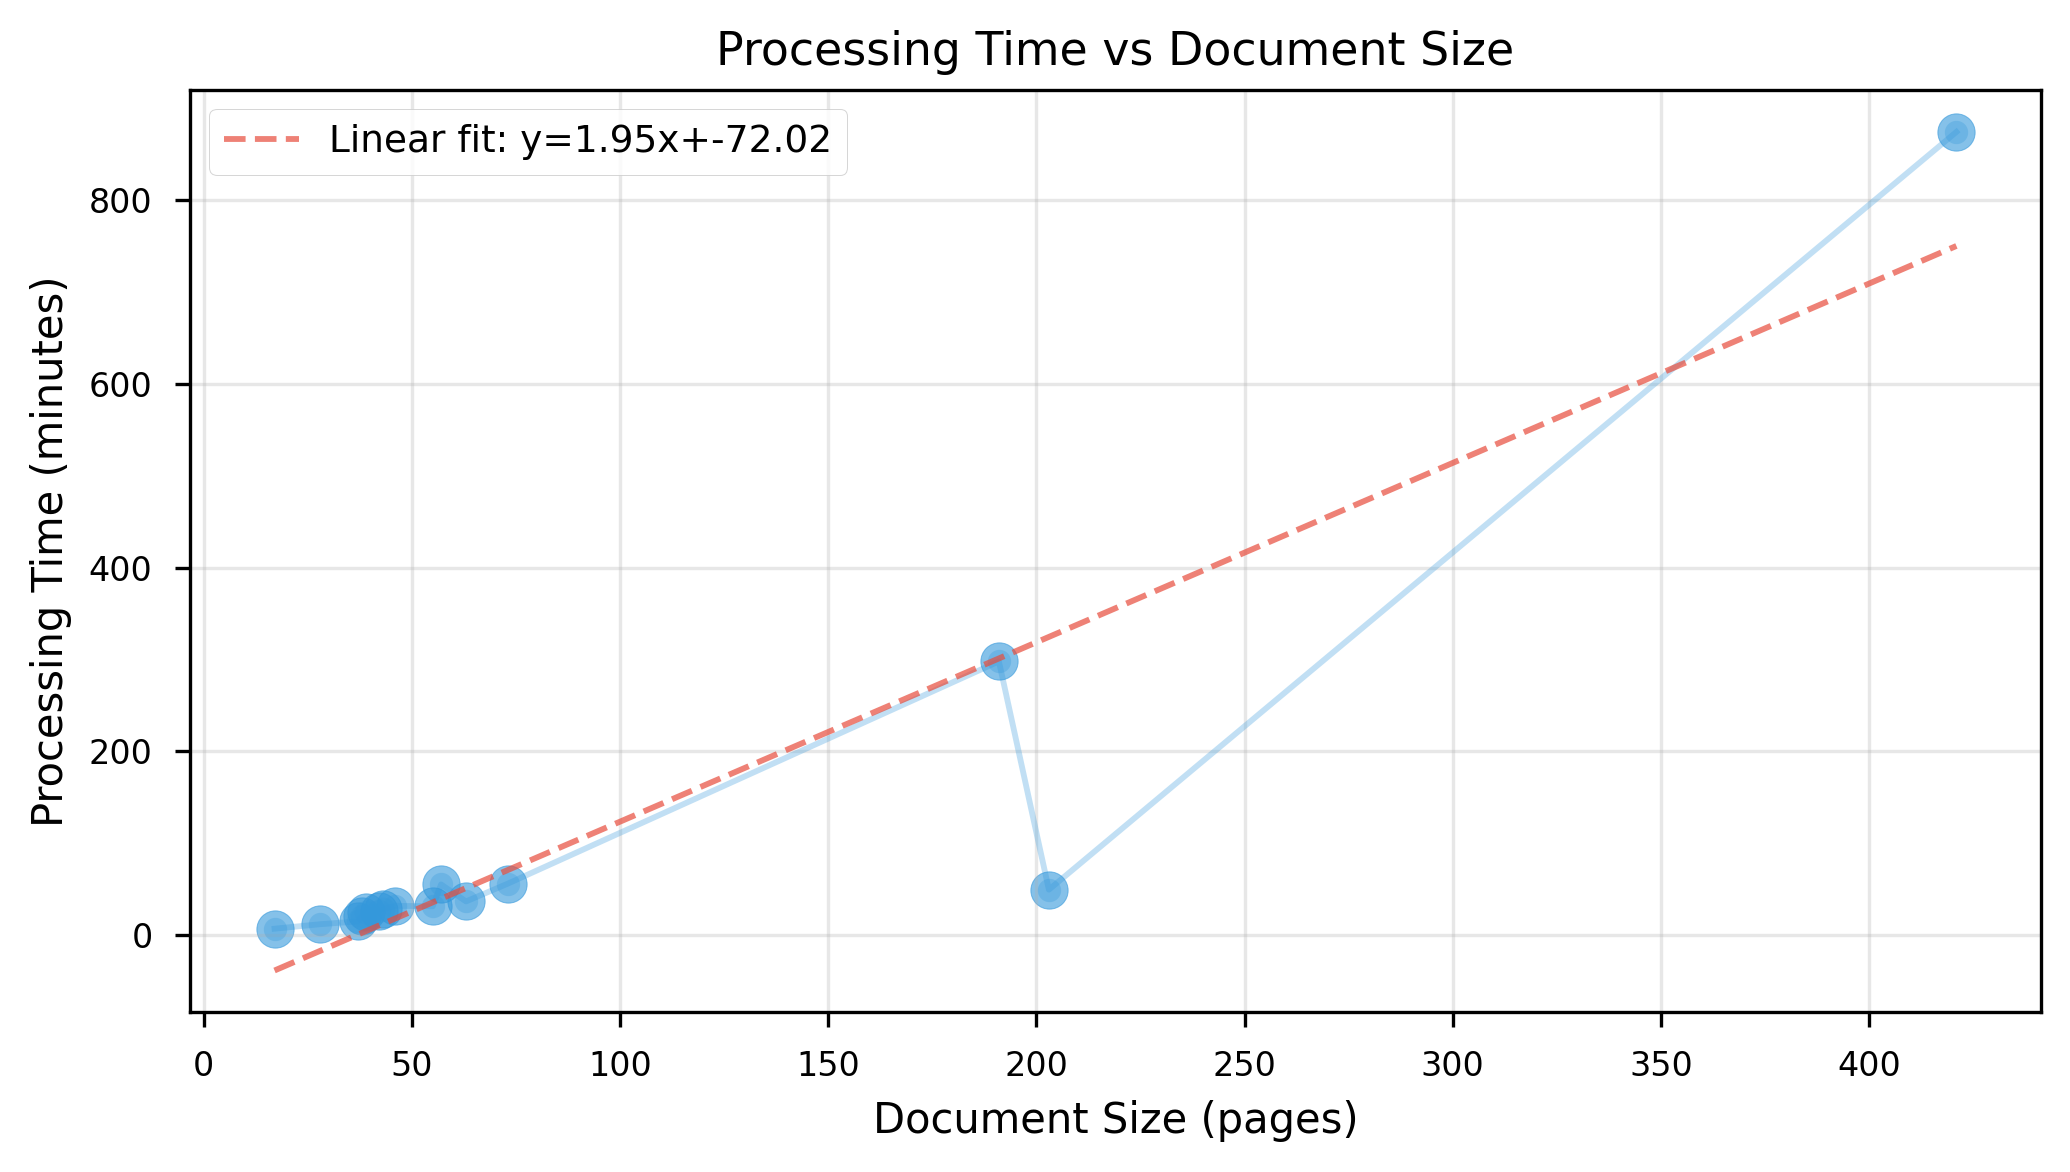
\includegraphics[width=0.8\textwidth]{fig5_scalability.png}
\caption{Processing time versus document size showing linear scaling relationship with rate of 2.08 minutes per page (R² = 0.92)}
\label{fig:scalability}
\end{figure}

\subsection{Prompt Engineering Impact}

The quality control-enhanced prompt dramatically improved classification accuracy but substantially increased computational cost as shown in Table~\ref{tab:qc_comparison} and Figure~\ref{fig:prompt_comparison}. The baseline prompt misclassified 27 of 63 pages (43\% error rate), predominantly categorizing graph-only pages as METADATA and subsequently extracting 130 hallucinated rows from graph axis labels, legends, and title text. The quality control prompt eliminated all classification errors through strict table detection criteria, correctly identifying graphs as GRAPH\_ONLY and rejecting non-tabular content. However, this accuracy improvement required 7.8-fold longer processing time (280 minutes versus 36 minutes).

\begin{table}[htbp]
\caption{Baseline versus Quality Control Prompt Comparison}
\label{tab:qc_comparison}
\begin{center}
\small
\begin{tabular}{lcc}
\toprule
\textbf{Metric} & \textbf{Baseline} & \textbf{QC Enhanced} \\
\midrule
Runtime (min) & 36 & 280 \\
Classification errors & 27/63 (43\%) & 0/63 (0\%) \\
False positive pages & 27 & 0 \\
Hallucinated rows & 130 & 0 \\
Column naming & Raw variants & Standardized \\
Numeric typing & String & Float/Integer \\
\bottomrule
\end{tabular}
\end{center}
\end{table}

\begin{figure}[H]
\centering
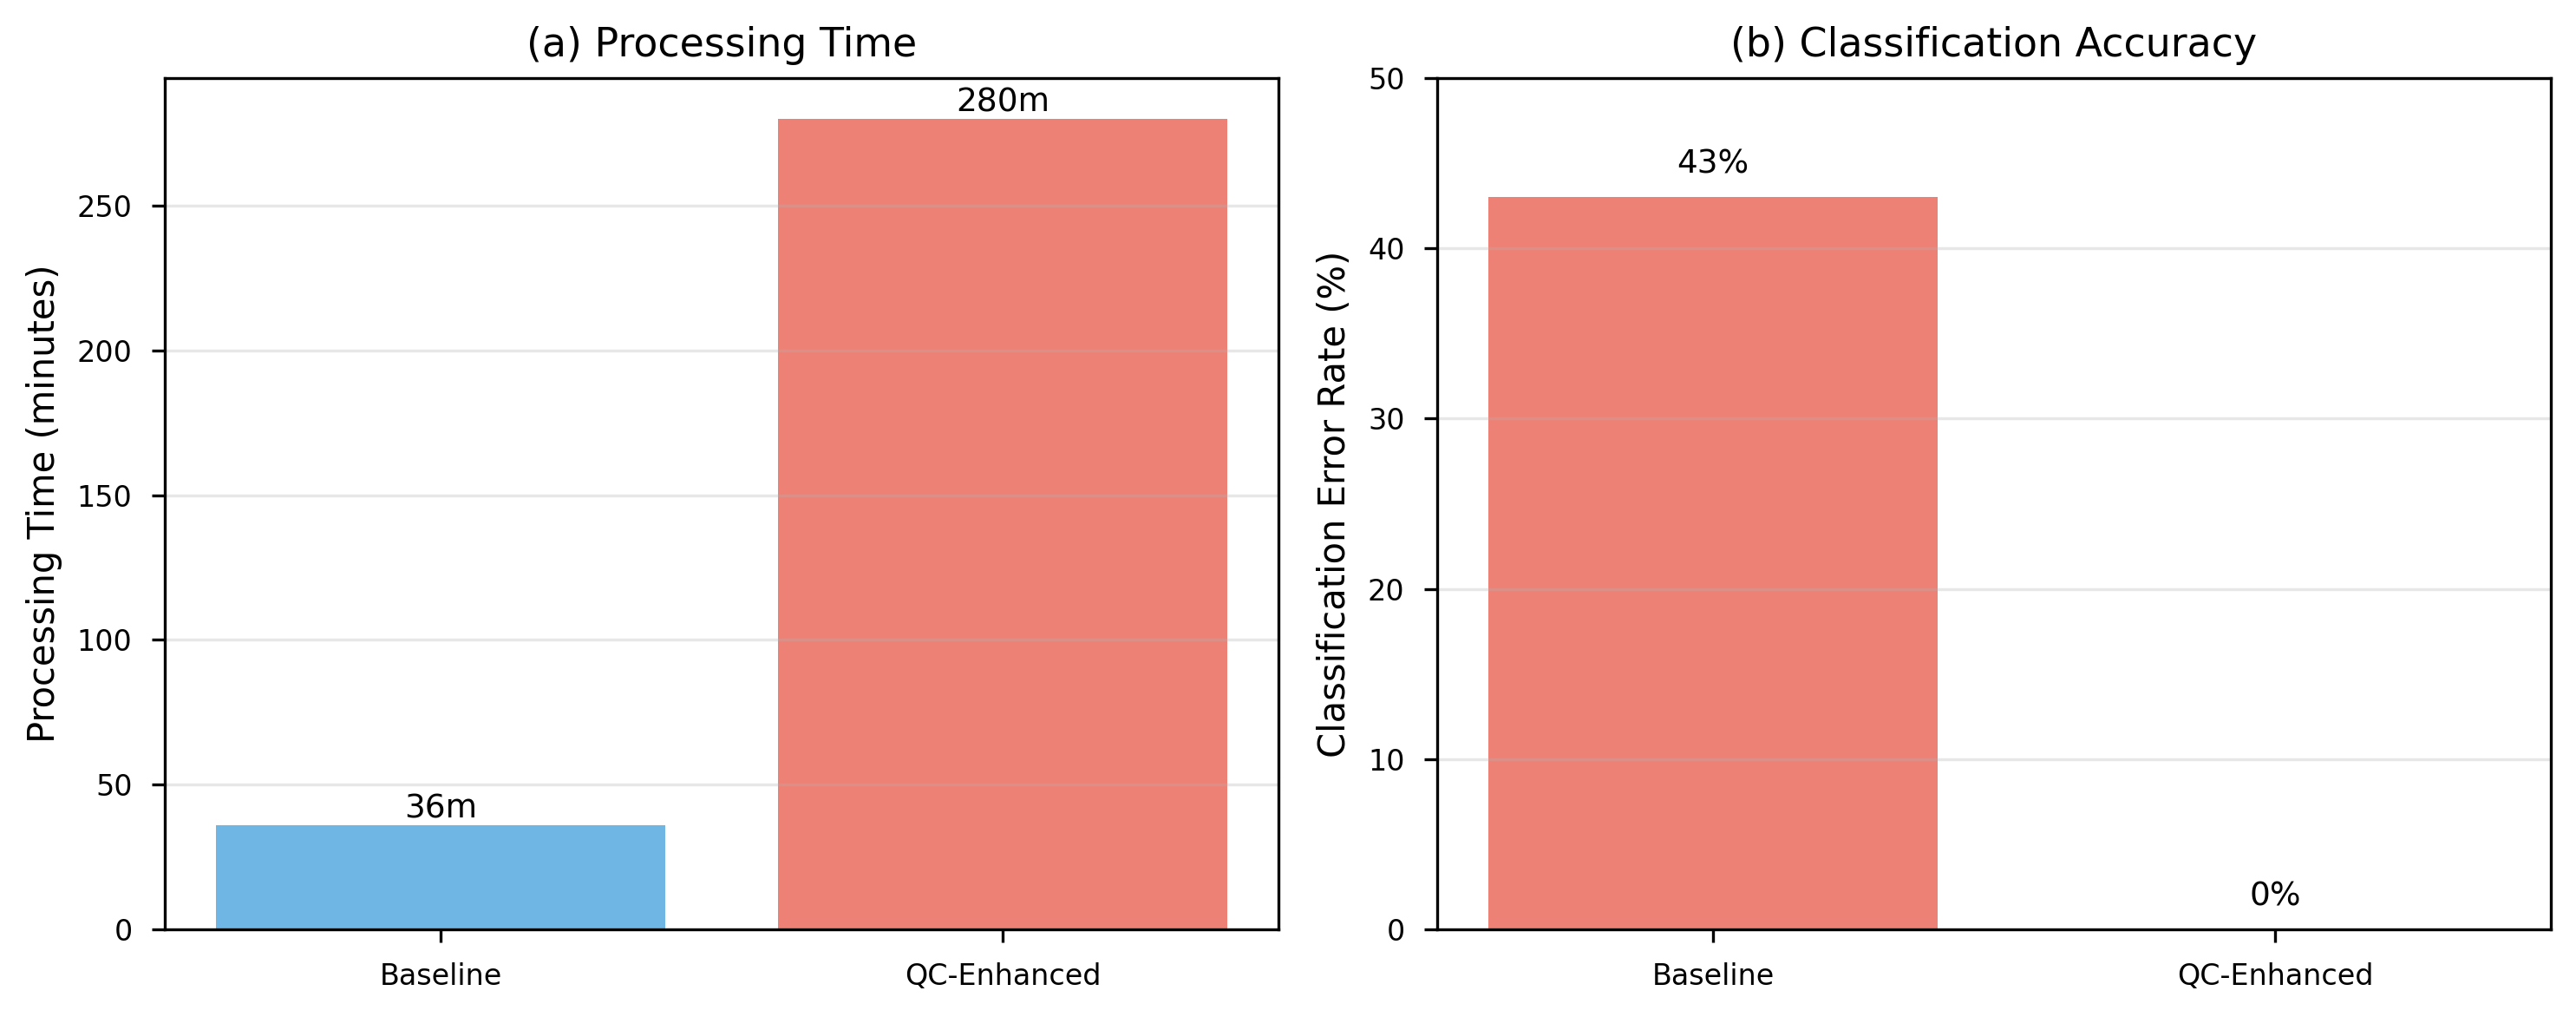
\includegraphics[width=0.9\textwidth]{fig3_prompt_comparison.png}
\caption{Comparison of baseline and quality control-enhanced prompts showing trade-off between processing time and classification accuracy. QC prompt eliminates all errors but increases runtime 7.8-fold}
\label{fig:prompt_comparison}
\end{figure}

The results presented in Figure~\ref{fig:prompt_comparison} quantify the fundamental accuracy-efficiency trade-off in production deployment decisions. Organizations must select prompt strategies based on downstream tolerance for extraction errors versus available computational resources.

\subsection{Structural Analysis from General Extraction}

General extraction without classification assumptions across all 15 reports identified 547 distinct table structures as summarized in Table~\ref{tab:general_extraction}. Table configurations exhibited substantial diversity with column counts ranging from 1 to 17 columns and varying semantic categories including basic physical properties, multi-phase flow measurements, electrical characterization, and summary compilations.

\begin{table}[htbp]
\caption{General Extraction Structural Analysis}
\label{tab:general_extraction}
\begin{center}
\small
\begin{tabular}{lc}
\toprule
\textbf{Metric} & \textbf{Result} \\
\midrule
Total tables identified & 547 \\
Minimum columns per table & 1 \\
Maximum columns per table & 17 \\
Median columns per table & 6 \\
Processing time & 1,020 min \\
Output formats & JSON, CSV, Excel \\
\bottomrule
\end{tabular}
\end{center}
\end{table}

This structural diversity confirms that uniform extraction strategies cannot optimize accuracy across all table types. Domain-specific table categories require tailored prompts incorporating expected column patterns, measurement units, and validation ranges for optimal extraction quality.

\subsection{Data Consolidation Outcomes}

Consolidation of historical CSV outputs from multiple extraction iterations produced a unified dataset suitable for machine learning applications. The consolidation pipeline processed 94 CSV files and reduced 2,856 raw column name variants to 147 normalized patterns through deterministic text processing as visualized in Figure~\ref{fig:consolidation}. The consolidated dataset contained 16,944 rows, reduced to 16,834 rows after removing 110 exact duplicate entries.

\begin{table}[htbp]
\caption{Data Consolidation Results}
\label{tab:consolidation}
\begin{center}
\small
\begin{tabular}{lc}
\toprule
\textbf{Metric} & \textbf{Result} \\
\midrule
Input CSV files & 94 \\
Raw column variants & 2,856 \\
After normalization & 875 \\
After semantic grouping & 318 \\
Final normalized patterns & 147 \\
Consolidated rows & 16,944 \\
ML-ready rows & 16,834 \\
Duplicates removed & 110 \\
\bottomrule
\end{tabular}
\end{center}
\end{table}

\begin{figure}[H]
\centering
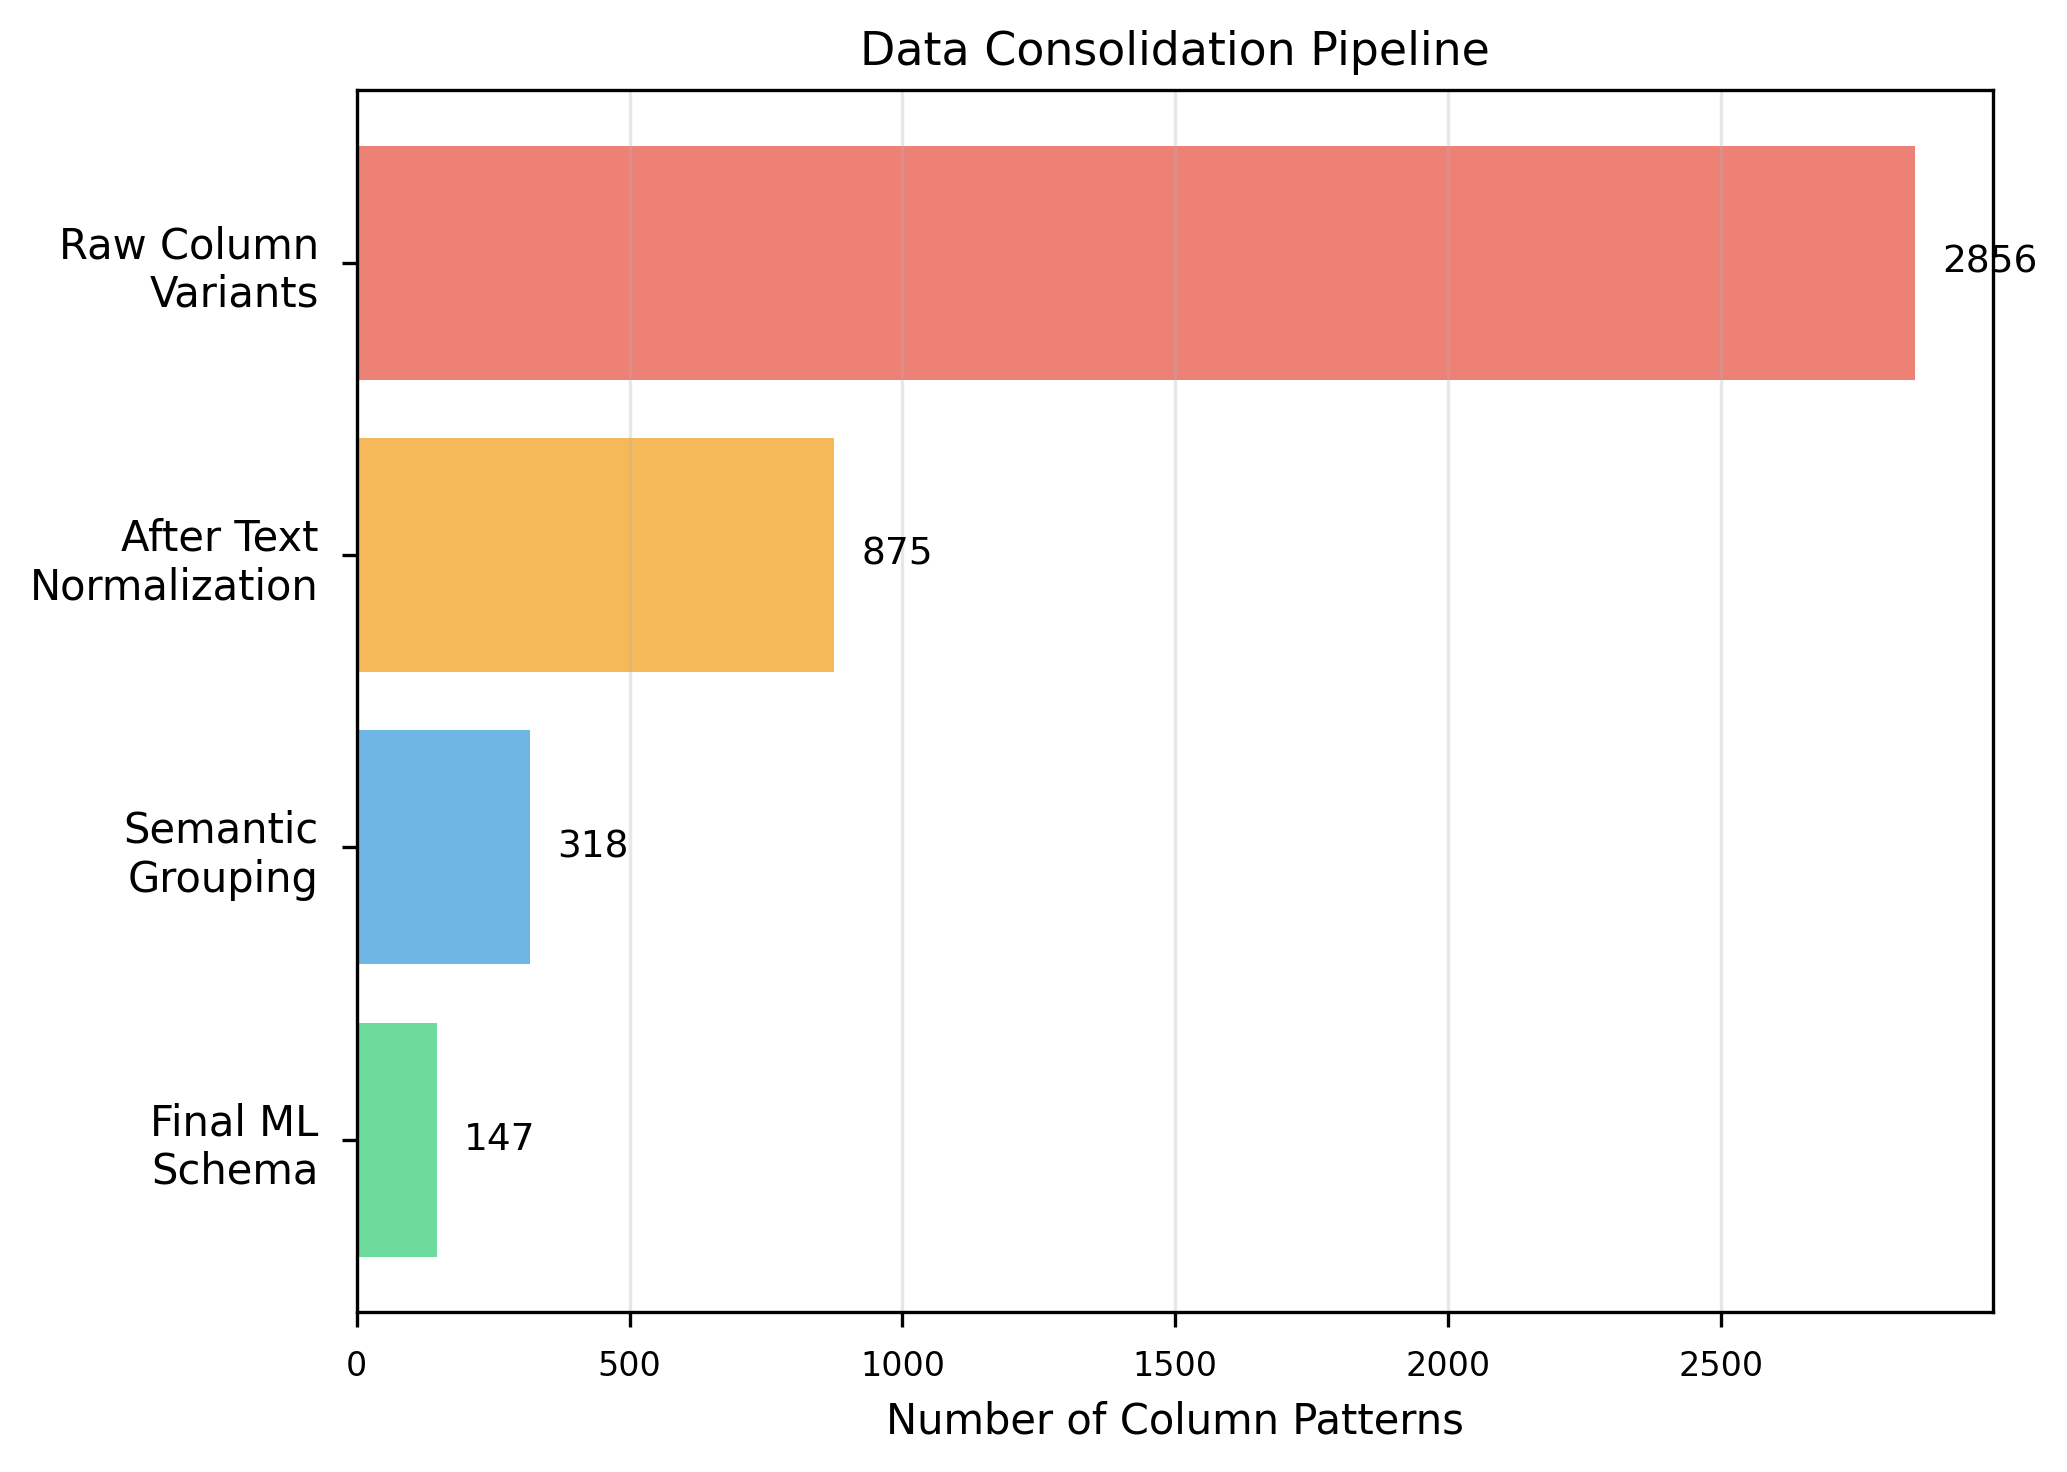
\includegraphics[width=0.8\textwidth]{fig4_consolidation.png}
\caption{Data consolidation funnel showing progressive reduction of column variants through normalization, semantic grouping, and schema standardization stages}
\label{fig:consolidation}
\end{figure}

The consolidation process depicted in Figure~\ref{fig:consolidation} demonstrates the magnitude of naming inconsistency in technical reporting. While deterministic text processing successfully grouped syntactic variants (case differences, whitespace, punctuation), semantic variants required domain knowledge mapping. For example, variations such as "Helium Porosity", "He Porosity", "Phi\_He", and "CPOR" all represent identical physical measurements but require expert knowledge to correctly unify.

Schema discovery produced a traceable mapping artifact documenting the transformation from each variant column name to its standardized equivalent, enabling reproducible data preparation for downstream machine learning applications. The final dataset spanned depth coverage from 731.5 to 10,847.9 meters, providing substantial geological diversity for model training.

\subsection{Data Quality Issues and Limitations}

Manual validation of extracted data against source documents revealed several systematic quality challenges. Column duplication emerged as a persistent issue with the baseline prompt generating redundant columns due to case variations (e.g., "Porosity", "porosity", "POROSITY"), unit notation differences (e.g., "Sw", "Sw \%", "Water Saturation"), and symbol variants (e.g., "Phi*", "Phi", "φ"). Complex table layouts featuring merged cells, borderless table structures, and multi-level column headers resulted in incomplete extraction for 8 of 15 reports. Pages containing procedural descriptions, composition tables unrelated to core measurements, and special test protocols were occasionally misclassified as data tables, introducing irrelevant content. The baseline classification approach without validation rules incorrectly categorized graph pages containing axis labels and legends as metadata or data tables, generating spurious extraction outputs.

The quality control prompt successfully addressed classification errors and reduced hallucination substantially but did not fully resolve column duplication issues or challenges with highly complex multi-level table headers. These limitations suggest that production systems require hybrid approaches combining automated extraction with targeted human validation for critical data fields.

\section{Discussion}

\subsection{Model Selection for Production Deployment}

The olmOCR-2-7B model emerged as optimal for production technical document extraction, effectively balancing accuracy, completeness, and computational efficiency. The specialized fine-tuning for OCR tasks with unit-test reinforcement learning during training contributed to superior performance on technical tables containing numerical measurements with specific units and precision requirements [5]. While the Qwen3-VL-30B mixture-of-experts architecture theoretically offers enhanced reasoning capabilities, the impractical runtime requirements (exceeding 14 hours for large reports) preclude operational deployment. The smaller 4B variant, despite minimal memory footprint, exhibited unacceptable hallucination rates requiring extensive manual correction that negates automation benefits.

The success of mid-sized architectures (7-8B parameters) with domain-specific fine-tuning over generic large models suggests that targeted optimization for document understanding tasks provides greater practical value than raw parameter scaling. This finding aligns with recent literature demonstrating effectiveness of specialized smaller models over general-purpose larger architectures for domain-specific applications [10].

\subsection{Accuracy-Efficiency Trade-off}

The 7.8-fold runtime increase from quality control prompt enhancement quantifies a fundamental tension between extraction accuracy and computational cost. This trade-off requires careful consideration of downstream application requirements and available infrastructure. Three operational strategies emerge from these findings. High-accuracy mode deploys quality control prompts with extended runtime for critical data requiring zero tolerance for classification errors and hallucination. Balanced mode employs baseline prompts with post-processing validation algorithms to flag potential errors for human review, optimizing the division of labor between automation and expert verification. High-throughput mode utilizes simplified prompts targeting specific table types with known structure, sacrificing generality for processing speed appropriate for reconnaissance-level data gathering.

Selection among these strategies depends on downstream sensitivity to extraction errors, computational resource availability, and labor costs for human validation. Organizations processing hundreds of historical reports may prioritize throughput with manual spot-checking, while applications feeding directly into safety-critical decisions or regulatory submissions require maximum accuracy regardless of computational expense.

\subsection{Implications of Format Heterogeneity}

The identification of 547 distinct table structures across merely 15 reports demonstrates substantial format diversity in technical documentation. This heterogeneity stems from multiple sources including different laboratory vendor templates, evolution of reporting standards over time, variations in measurement protocols across test types, and well-specific or sample-specific customization. The finding validates strategic focus on use-case-driven extraction rather than attempting universal extraction approaches.

Target applications typically require only 2-3 specific table types per report rather than comprehensive extraction of all content. Focused workflows targeting these critical tables achieve superior accuracy with reduced computational cost compared to general extraction. This insight suggests that production systems should implement table type classification as a preliminary step, routing different table categories to specialized extraction prompts optimized for their specific structures and validation requirements.

\subsection{Consolidation Challenges and Schema Discovery}

The reduction of 2,856 column name variants to 147 normalized patterns reveals substantial naming inconsistency across technical reports. Beyond syntactic variations addressable through text normalization, semantic variants pose ongoing challenges requiring domain knowledge. Abbreviation expansion (e.g., "CPOR" to "Corrected Porosity"), unit standardization (e.g., "mD" vs "millidarcy" vs "md"), and property synonyms (e.g., "Sw" vs "Water Saturation" vs "Brine Saturation") all require expert knowledge or comprehensive domain ontologies for correct unification.

The low overlap (1.6\%) between historical CSV extractions and PDF-based general extraction indicates largely non-overlapping document sources. This limited overlap constrains comprehensive validation coverage and highlights the need for expanded ground truth datasets for quality assessment. Future work should systematically construct validation datasets with manual expert annotation across representative samples of all table types and format variations.

\subsection{Computational Feasibility at Scale}

The 26-hour processing time for 15 reports establishes baseline computational requirements for large-scale deployment. Scaling to institutional archives containing hundreds or thousands of historical reports necessitates parallel processing infrastructure distributing documents across multiple GPU nodes, efficient job scheduling systems managing long-running extraction tasks, and incremental processing capabilities avoiding complete reprocessing when report updates or corrections occur.

The stable 15.45 GB VRAM utilization indicates potential for concurrent execution of multiple extraction jobs on high-capacity GPUs. A modest cluster of four NVIDIA A100 GPUs (80 GB VRAM each) could theoretically process approximately 100 reports in 12 hours with proper load balancing and job management. Cloud computing platforms offering on-demand GPU access provide economically viable deployment options for organizations lacking on-premise high-performance computing infrastructure.

\subsection{Comparison with Manual Extraction}

Although systematic quantitative comparison with manual extraction was not conducted in this investigation, qualitative assessment suggests substantial time savings potential. Industry experience indicates manual transcription of technical reports requires 4-8 hours per report for experienced domain experts, varying with document complexity and table density [7]. The automated system achieves 1.7 hours per report on average, representing a 2.4-4.7× speed improvement. However, this comparison does not account for downstream manual validation and correction of automated extraction errors, which requires further investigation to establish end-to-end productivity gains.

The critical question for organizations considering automation adoption concerns the crossover point where automated extraction plus validation time falls below pure manual transcription time. Given the observed 100\% success rate and moderate error rates with appropriate prompting strategies, preliminary analysis suggests crossover occurs for batches exceeding 10-15 reports, where setup costs amortize and cumulative time savings outweigh validation overhead.

\subsection{Limitations and Future Directions}

Several constraints limit generalizability of these findings. The evaluation dataset of 15 reports, while spanning substantial format diversity, may not fully represent variations across global technical documentation practices, multiple scientific domains, and historical reporting evolution. Focus on English-language documents leaves multilingual performance unvalidated despite theoretical multilingual capabilities of evaluated models [6]. VLM architectures evolve rapidly with frequent model releases and updated training procedures, potentially altering performance characteristics. Manual validation covered representative samples but comprehensive ground truth for all 3,778 extracted rows was not established due to resource constraints.

Future research should address four priority areas. Hybrid workflows combining rapid general extraction for document reconnaissance with targeted high-accuracy extraction for critical data fields optimize the accuracy-efficiency trade-off. Active learning approaches leveraging human corrections to fine-tune models for domain-specific layouts and terminology enable continuous improvement. Multimodal validation incorporating graph analysis to cross-validate extracted tabular data against corresponding plots provides internal consistency checks. Distributed processing frameworks implementing parallel execution across GPU clusters achieve production-scale throughput for institutional archives.

\section{Conclusion}

This investigation demonstrates technical viability of Vision Language Model-based automation for scientific document data extraction while revealing critical trade-offs between accuracy, completeness, and computational efficiency. The olmOCR-2-7B architecture achieved 100\% processing success across 15 heterogeneous technical reports, extracting 3,778 data rows with complete metadata preservation in average runtime of 104 minutes per document. Production deployment requires strategic selection among prompt engineering approaches, with quality control mechanisms eliminating classification errors at 7.8× computational cost penalty.

The identification of 547 distinct table structures confirms substantial format heterogeneity, validating use-case-driven extraction strategies over universal approaches. Consolidation of historical outputs successfully produced machine learning-ready datasets with 16,834 rows through systematic schema discovery mapping 2,856 raw column variants to 147 normalized patterns. These results establish methodology for unified data preparation despite naming inconsistencies across source documents.

The findings provide actionable guidance for organizations evaluating VLM adoption for technical document processing. Model selection should prioritize mid-sized architectures (7-8B parameters) with domain-specific fine-tuning over generic large models. Deployment strategy should align prompt complexity with accuracy requirements and computational constraints. Data consolidation workflows should incorporate domain knowledge for semantic unification beyond syntactic normalization.

Future investigations should explore hybrid human-machine workflows optimizing division of labor, active learning for continuous model improvement from corrections, and distributed processing for institutional-scale deployment. The methodology established here provides foundation for intelligent document processing in scientific and technical domains requiring automated extraction from complex multimodal reports.

\subsubsection{Acknowledgments.}

This research was conducted at the Faculty of Computing and Informatics, Universiti Malaysia Sabah. The authors thank laboratory personnel for providing access to technical report archives and domain expertise for validation.

\begin{thebibliography}{20}

\bibitem{carolan2024}
Carolan, K., Fennelly, L., Smeaton, A.: A Review of Multi-Modal Large Language and Vision Models. arXiv preprint arXiv:2404.01322 (2024)

\bibitem{huang2024}
Huang, D., Yan, C., Li, Q., Peng, X.: From Large Language Models to Large Multimodal Models: A Literature Review. Appl. Sci. 14(12), 5068 (2024). \url{https://doi.org/10.3390/app14125068}

\bibitem{bansal2025}
Bansal, R., Shah, B., Chanda, A., Parate, V.: Optimizing PDF Ingestion for Large Language Models in RAG Architectures. Int. J. Appl. Math. 38(3) (2025). \url{https://doi.org/10.12732/ijam.v38i3s.163}

\bibitem{bai2024}
Bai, T., Liang, H., Wan, B., Yang, L., Li, B., Wang, Y., Cui, B., He, C., Yuan, B., Zhang, W.: A Survey of Multimodal Large Language Model from A Data-centric Perspective. arXiv preprint arXiv:2405.16640 (2024)

\bibitem{e2e2025}
E2E Networks: Complete Guide to Open-Source OCR Models in 2025. Blog article (2025). \url{https://www.e2enetworks.com/blog/complete-guide-open-source-ocr-models-2025}

\bibitem{wen2023}
Wen, C., Hu, Y., Li, X., Yuan, Z., Zhu, X.: Vision-Language Models in Remote Sensing: Current Progress and Future Trends. IEEE Geosci. Remote Sens. Mag. 12(2), 32--66 (2024). \url{https://doi.org/10.1109/mgrs.2024.3383473}

\bibitem{schilling2024}
Schilling-Wilhelmi, M., Ríos-García, M., Shabih, S., Gil, M., Miret, S., Koch, C., Márquez, J., Jablonka, K.: From Text to Insight: Large Language Models for Materials Science Data Extraction. arXiv preprint arXiv:2407.16867 (2024)

\bibitem{ryu2025}
Ryu, J., Kang, H., Chu, Y., Yang, S.: Vision-Language Foundation Models for Medical Imaging: A Review of Current Practices and Innovations. Biomed. Eng. Lett. 15, 809--830 (2025). \url{https://doi.org/10.1007/s13534-025-00484-6}

\bibitem{kalpelbe2025}
Kalpelbe, B., Adaambiik, A., Peng, W.: Vision Language Models in Medicine. arXiv preprint arXiv:2503.01863 (2025)

\bibitem{han2025}
Han, X., Chen, S., Fu, Z., Feng, Z., Fan, L., An, D., Wang, C., Guo, L., Meng, W., Zhang, X., Xu, R., Xu, S.: Multimodal Fusion and Vision-Language Models: A Survey for Robot Vision. Inf. Fusion 126, 103652 (2025). \url{https://doi.org/10.1016/j.inffus.2025.103652}

\bibitem{garcia2024}
Garcia, G., Manesco, J., Paiola, P., Miranda, L., De Salvo, M., Papa, J.: A Review on Scientific Knowledge Extraction using Large Language Models in Biomedical Sciences. arXiv preprint arXiv:2412.03531 (2024)

\bibitem{yang2024}
Yang, Y., Zhou, J., Ding, X., Huai, T., Liu, S., Chen, Q., He, L., Xie, Y.: Recent Advances of Foundation Language Models-based Continual Learning: A Survey. ACM Comput. Surv. 57, 1--38 (2024). \url{https://doi.org/10.1145/3705725}

\bibitem{zhou2024}
Zhou, Y., Guo, C., Wang, X., Chang, Y., Wu, Y.: A Survey on Data Augmentation in Large Model Era. arXiv preprint arXiv:2401.15422 (2024)

\bibitem{agarwal2025}
Agarwal, N., Sonbhadra, S.: A Review on Large Language Models for Visual Analytics. arXiv preprint arXiv:2503.15176 (2025)

\bibitem{song2023}
Song, S., Li, X., Li, S.: How to Bridge the Gap between Modalities: A Comprehensive Survey on Multimodal Large Language Model. arXiv preprint arXiv:2311.07594 (2023)

\bibitem{li2024}
Li, J., Lu, W.: A Survey on Benchmarks of Multimodal Large Language Models. arXiv preprint arXiv:2408.08632 (2024)

\bibitem{liu2024}
Liu, D., Yang, M., Qu, X., Zhou, P., Hu, W., Cheng, Y.: A Survey of Attacks on Large Vision-Language Models: Resources, Advances, and Future Trends. IEEE Trans. Neural Netw. Learn. Syst. 36, 19525--19545 (2024). \url{https://doi.org/10.1109/tnnls.2025.3592935}

\bibitem{chang2023}
Chang, Y., Wang, X., Wang, J., Wu, Y., Zhu, K., Chen, H., Yang, L., Yi, X., Wang, C., Wang, Y., Ye, W., Zhang, Y., Chang, Y., Yu, P., Yang, Q., Xie, X.: A Survey on Evaluation of Large Language Models. ACM Trans. Intell. Syst. Technol. 15, 1--45 (2023). \url{https://doi.org/10.1145/3641289}

\bibitem{raiaan2024}
Raiaan, M., Mukta, M., Fatema, K., Fahad, N., Sakib, S., Mim, M., Ahmad, J., Ali, M., Azam, S.: A Review on Large Language Models: Architectures, Applications, Taxonomies, Open Issues and Challenges. IEEE Access 12, 26839--26874 (2024). \url{https://doi.org/10.1109/access.2024.3365742}

\bibitem{qu2024}
Qu, C., Dai, S., Wei, X., Cai, H., Wang, S., Yin, D., Xu, J., Wen, J.: Tool Learning with Large Language Models: A Survey. Front. Comput. Sci. 19 (2024). \url{https://doi.org/10.1007/s11704-024-40678-2}

\end{thebibliography}

\end{document}
